\chapter{Descrizione del sistema}
\label{scenario}
Data la complessità del sistema ideato utilizzeremo un approccio top-down per descriverlo. Partendo da un livello di astrazione tale da descrivere i macro requisiti funzionali, concluderemo il capitolo dettagliando le parti del sistema realizzate nel contesto di questa tesi.


\section{Requisiti funzionali}
Considerando il sistema in questione come una black-box e l'infrastruttura di rete in modo astratto, i due macro-requisiti funzionali (rappresentati in Fig.\ref{fig:requisitiFunzionali}) sono rispettivamente:
\begin{itemize}
	\item \textbf{R1: Geolocalizzazione dell'operatore}
	\item \textbf{R2: Trasmissione di messaggi predefiniti} come stato della vittima, codici d'emergenza etc etc.
\end{itemize}
 Questi costituiscono la base di partenza di progettazione ma sopratutto il punto di arrivo del progetto stesso. \\
\begin{figure}[H]
	\centering
	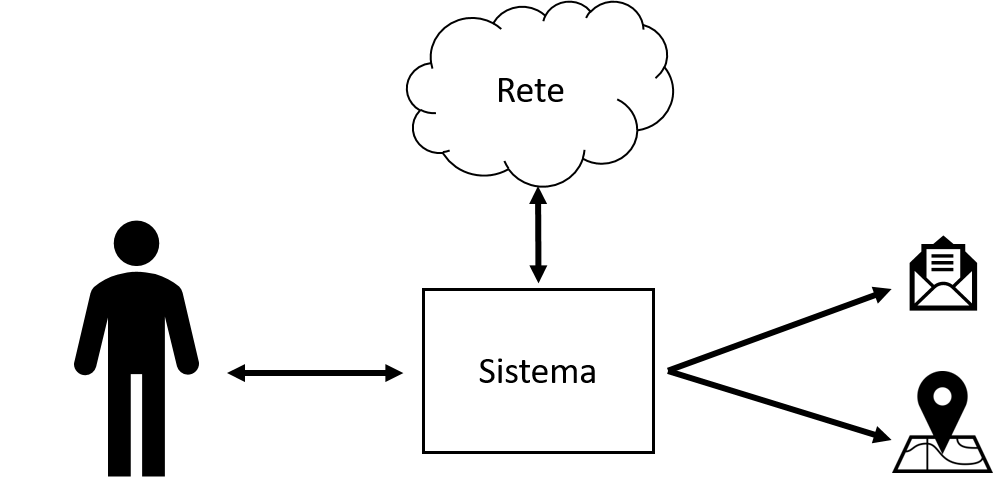
\includegraphics[scale=0.3]{DescrizioneDelSistema/requisitiSistema.png}
	\caption{Rappresentazione figurale dei requisiti funzionali del sistema }
	\label{fig:requisitiFunzionali}
\end{figure}
Nelle fasi primordiali del progetto, si è scelto di allocare la maggior parte delle risorse lavorative nel completamento di \textbf{R1} lasciando ad una fase successiva lo sviluppo di \textbf{R2}. Per questo motivo d'ora in avanti, considereremo come unico obiettivo la geolocalizzazione dell'operatore.\\
Andiamo quindi ad aprire la black-box rappresentante il sistema in Fig.\ref{fig:requisitiFunzionali} consi





\section{Il sistema realizzato}